\section{Analyse des Roboters}
\label{sec:analyse-des-roboters}
Dieses und die folgenden Kapitel beschäftigen sich lediglich mit der Infrastruktur rund um den Roboter
und der Hardware und den Funktionen, die bereits im Roboter verbaut sind oder ergänzt werden können.
Die Funktionen rund um \gls{ml}, erweiterte Robotik, \todo{abk} LIDAR werden nicht behandelt.
Dieses Kapitel beschäftigt sich mit dem Ansatz der Analyse des Roboters.
Es wird gezeigt, wie die bestehenden Funktionen getestet und genutzt werden können, wie erkannt wird,
welche Funktionen bereits aktiviert sind und welche Teile der Soft- oder Hardware nicht aktiviert sind.
Zum Abschluss werden die bereits vorhanden Funktionen in dem Umfang, in dem sie ab Werk geliefert wurden,
gezeigt und erklärt.
Einige der Funktionen werden im späteren Verlauf der Arbeit auch erweitert oder verändert.
Die Dokumentation hierzu ist in Kapitel~\ref{sec:funktionserweiterungen-und-integration} zu finden.
Betroffene Funktionen werden hier im Kapitel explizit hervorgehoben.



\subsection{Analytische Vorgehensweise}
\label{subsec:vorgehensweise}
% Was mache ich, wenn ich was rausfinden möchte?
% Welche Ansätze für unbekannte Funktionen
% Meistens funktionierende Ansätze

\subsection{Funktionen}
\label{subsec:funktionen}

Im folgenden Kapitel werden einige der im Werkszustand mitgelieferten Funktionen des \gls{go1} erklärt und vorgeführt.
Einige der Funktionen sind bereits freigeschaltet und bedürfen keiner bis weniger Konfiguration.
Andere sind nicht freigeschaltet oder kaum dokumentiert, weshalb diese detaillierter beschrieben werden.
Teile der Funktionen sind nicht im Umfang der Arbeit erfasst worden.
Alle bekannten nicht erfassten Funktionen werden am Ende des Kapitels aufgezählt.
\subsubsection{Fernsteuerung}
\label{subsubsec:fernsteuerung}
%todo fernbedienung in fernsteuerung

Der \gls{go1} lässt sich auf vier verschiedene Arten fernsteuern:

\begin{itemize}
    \item Fernbedienung
    \item App
    \item Webinterface
    \item Folgefunktion
\end{itemize}

\noindent Dieses Kapitel beschreibt alle vier Möglichkeiten kurz und zeigt diverse Limitierungen der einzelnen Umsetzungen auf.
Für alle vier Steuermöglichkeiten muss der Roboter angeschaltet und der Sportmodus aktiviert sein.
Sollte der Sportmodus nicht aktiviert sein und eine Verbindung auf den Raspberry Pi nicht möglich oder erwünscht sein,
so kann dieser über die gekoppelte Fernbedienung und der Tastenkombination \texttt{L2+START} aktiviert werden.
Der \gls{go1} muss sich hierfür in der Ausgangsposition wie in Kapitel \ref{subsubsec:inbetriebnahme_akku} beschrieben befinden.

\myparagraph{Fernbedienung}

Der Lieferumfang des \gls{go1} umfasst zwei physische Fernbedienungen, mit denen der Roboter gesteuert werden kann.
Die Hauptfernbedienung besitzt zwei sogenannte Joysticks, welche die Position und Bewegung Roboter in verschiedenen Achsen
manipulieren können.
Die zweite Fernbedienung, von Unitree \emph{Label Controller} genannt, besitzt lediglich ein Joystick, welches die Bewegung
nach vorne, hinten, links und rechts steuern kann.
Sie dient ebenfalls als Sender für die \emph{Folge}-Funktion.
Abbildung \ref{fig:controller} zeigt links die Hauptfernbedienung und rechts den Label-Controller.

\begin{figure}[h]
    \frame{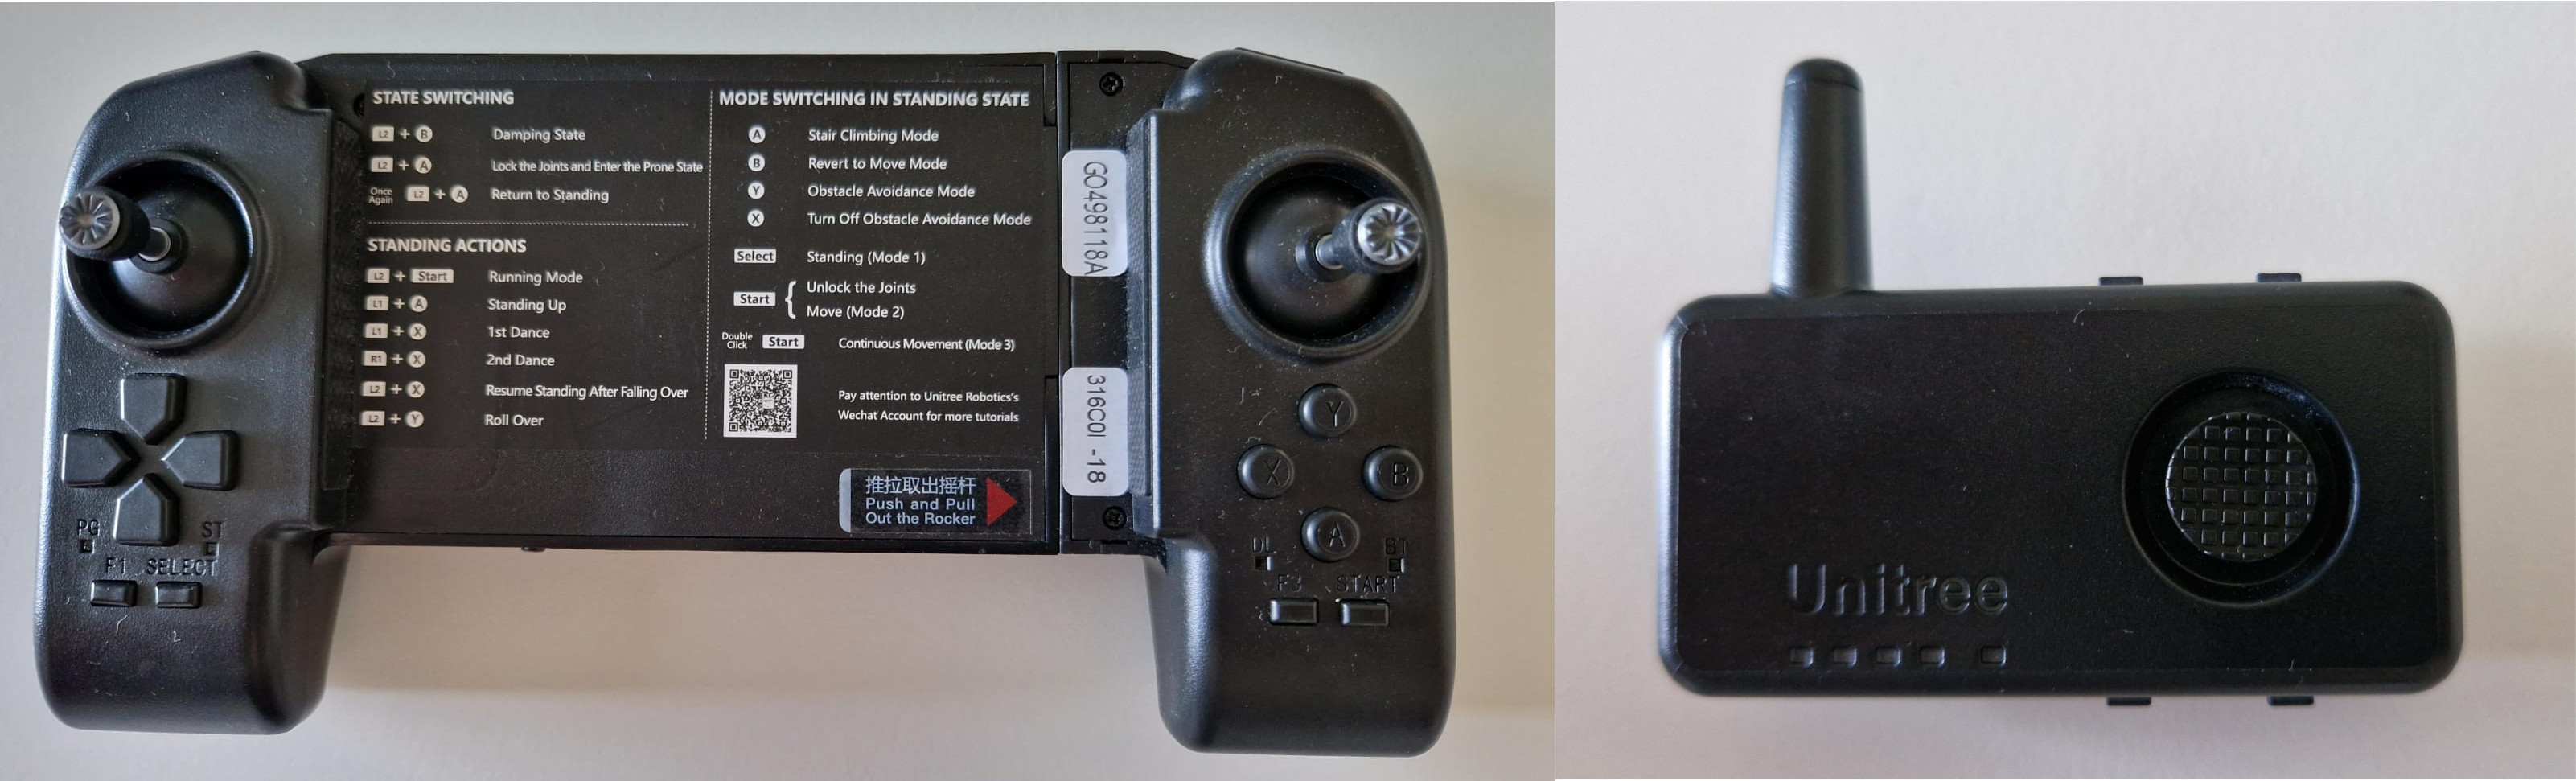
\includegraphics[width=\linewidth]{img/analyse/controller}}
    \caption{Hauptfernbedienung (links) und Label-Controller (rechts)}\label{fig:controller}
\end{figure}

Die einfache Bedienung der Hauptfernbedienung ist bereits nach dem Anschalten des Roboters nach Kapitel \ref{subsubsec:inbetriebnahme_akku} möglich.
Hierbei koppelt sich die Fernbedienung automatisch mit dem Roboter.
Dokumentation über die Art der Verbindung ist nicht auffindbar, es wird jedoch vermutet, dass dies nicht über Bluetooth,
sondern über ein anderes Protokoll geschieht und sich die Fernbedienung mit der \gls{mcu} statt mit dem Raspberry
Pi verbindet, welcher auch über Bluetooth verfügen würde.
Es beseht jedoch die Möglichkeit, die Fernbedienung via Bluetooth mit einem Smartphone zu koppeln.
Hierfür muss zur Verifikation der Kopplung der Pin \texttt{1234} verwendet werden.
Der Kopplungsprozess ist unter den verschiedenen Herstellern unterschiedlich und wird deshalb hier nicht weiter dokumentiert.
Nach erfolgreicher Kopplung kann über die mobile App\footnote{Siehe Kapitel \ref{subsubsec:anwendungen}} die Fernbedienung verbunden werden.
Über die Einstellungen und den Menüpunkt \texttt{Peripherals > Bluetooth Gamepad} kann in der Liste \texttt{Gamepad List}
die Fernbedienung mit der übereinstimmenden Seriennummer ausgewählt werden.
Diese ist ab Werk auf den Fernbedienungen gelabelt.
Abbildung \ref{fig:controller-app} zeigt die Bildschirmaufnahmen der relevanten Menüpunkte der App.

\begin{figure}[h]
    \frame{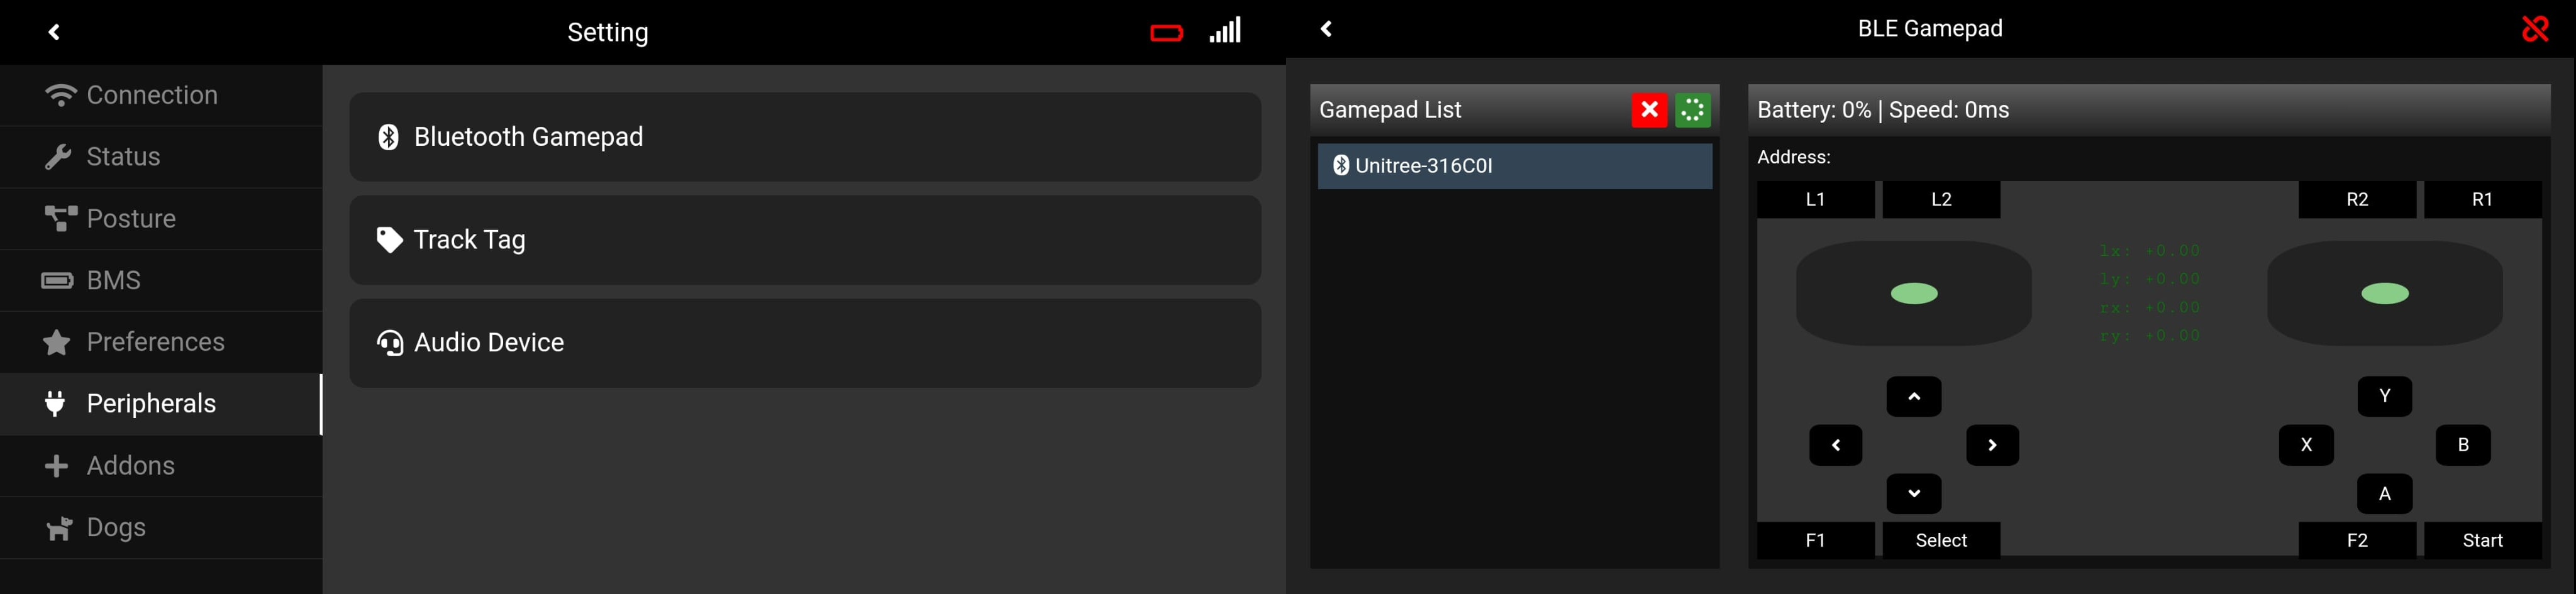
\includegraphics[width=\linewidth]{img/analyse/controller-app}}
    \caption{App-Menüpunkte \texttt{Peripherals > Bluetooth Gamepad} und \texttt{Gamepad List}}\label{fig:controller-app}
\end{figure}

\noindent Nun besteht die Möglichkeit, den \gls{go1} über die Fernbedienung fernzusteuern, egal in welchem Netzwerk er sich befindet.
Es ist lediglich notwendig, dass sich der Roboter und das Handy im selben Netzwerk befinden.
Weitere Informationen zur Netzwerkerweiterung sind in Kapitel \ref{sec:funktionserweiterungen-und-integration} dokumentiert.

\myparagraph{App}

Der \gls{go1} lässt sich ebenfalls durch die mobile Anwendung steuern, ohne sie vorher mit der Hauptfernbedienung verbunden zu haben.
Hierfür muss der Hauptmenüpunkt \texttt{Vision} ausgewählt werden.
Danach muss im rechten oberen Eck die Steuerung in der Ansicht der Kameras aktiviert werden.
Wie auf Abbildung \ref{fig:app-controller} gezeigt kann dann der Modus im rechten unteren Eck des Bildschirmes gewählt werden.
Wählt man hier einen der Laufmodi aus, so lässt sich der \gls{go1} mit den beiden dargestellten Steuereinheiten bewegen.
Links stellt die linke Steuereinheit der Hauptfernbedienung dar, rechts die rechte Einheit.

\begin{figure}[h]
    \frame{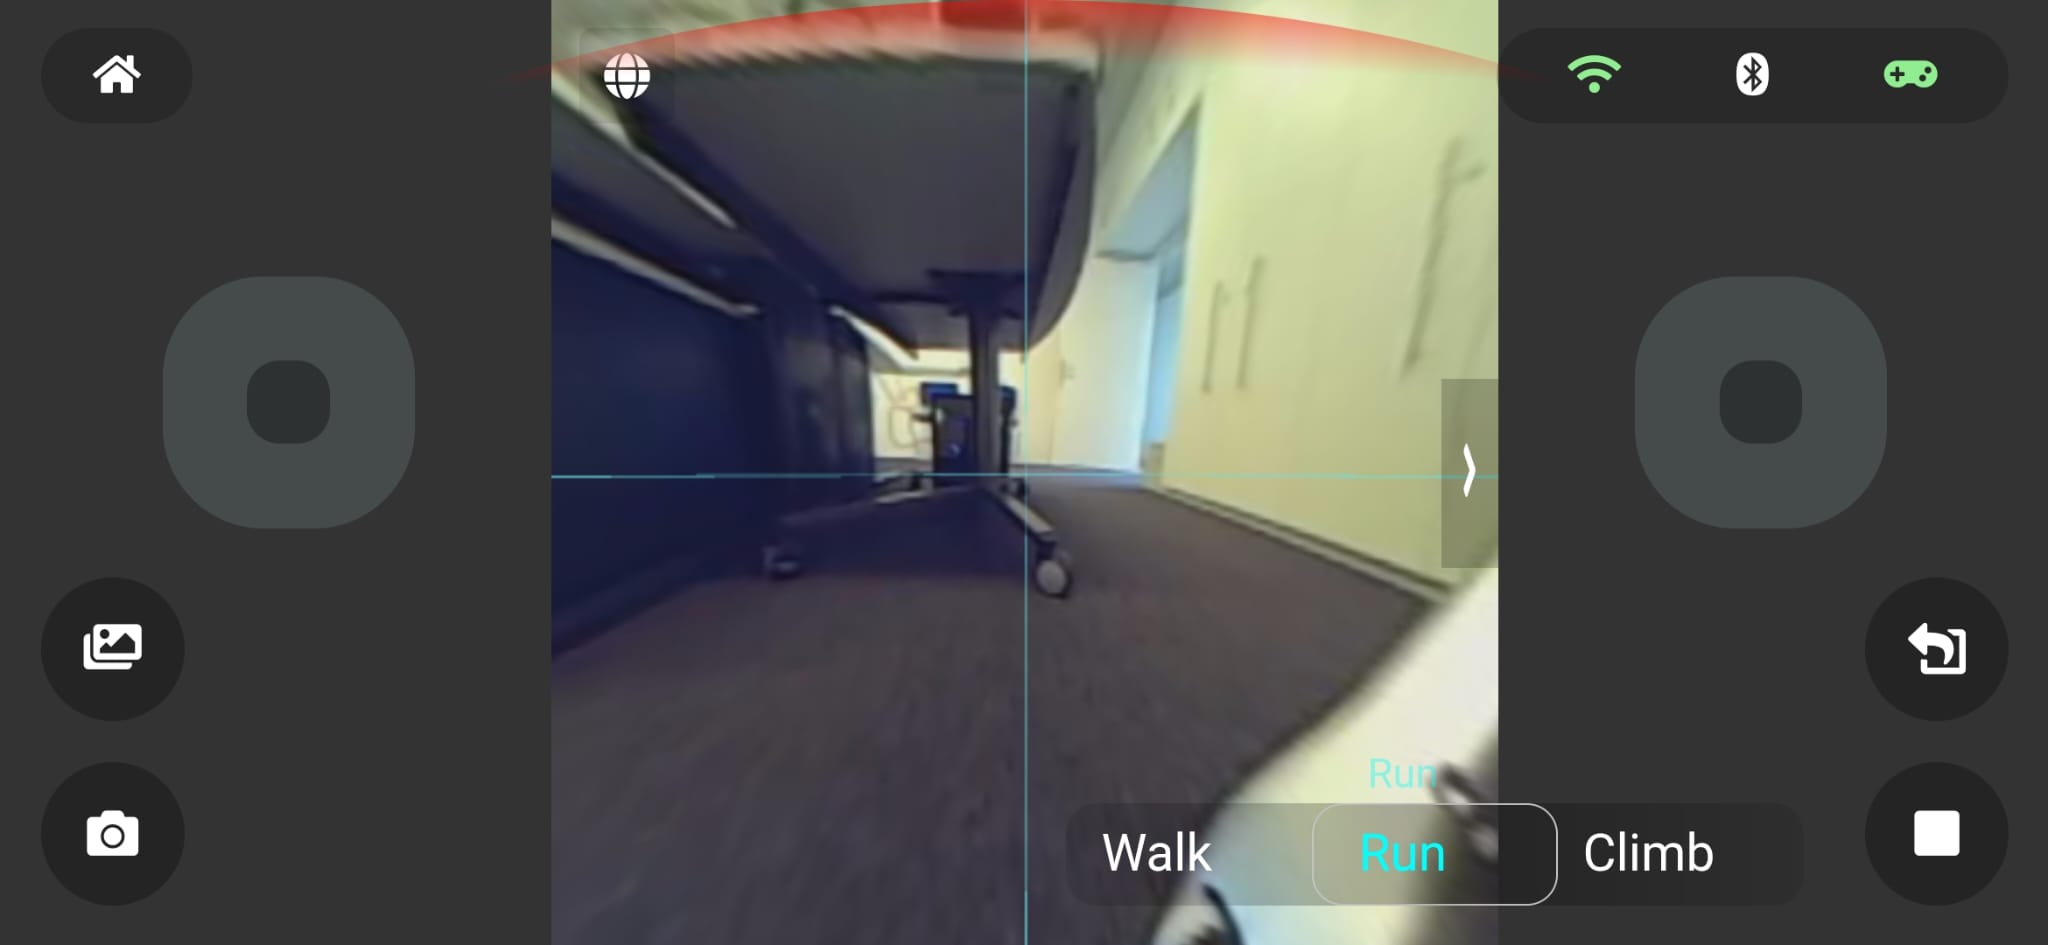
\includegraphics[width=\linewidth]{img/analyse/app-controller}}
    \caption{Bildschirmaufnahme des App-Controllers}\label{fig:app-controller}
\end{figure}

\myparagraph{Webinterface}

Die Webseite, die auf dem Raspberry Pi gehostet wird, bieter im Menü \texttt{Vision} die Möglichkeit, im rechten
oberen Eck des Bildschirmes die Steuerung des Roboters zu aktivieren.
Nach Aktivierung werden dem Nutzer, wie auf Abbildung \ref{fig:web-controller} dargestellt, zwei Steuerelemente dargestellt.
Diese können links mit den Tasten \texttt{W-A-S-D} und rechts mit den Tasten \texttt{\textuparrow -\textleftarrow -\textdownarrow -\textrightarrow}
gesteuert.
Die linke Steuereinheit entspricht der linken Seite der Hauptfernbedienung, die rechte dementsprechend der rechten Seite.

\begin{figure}[h]
    \frame{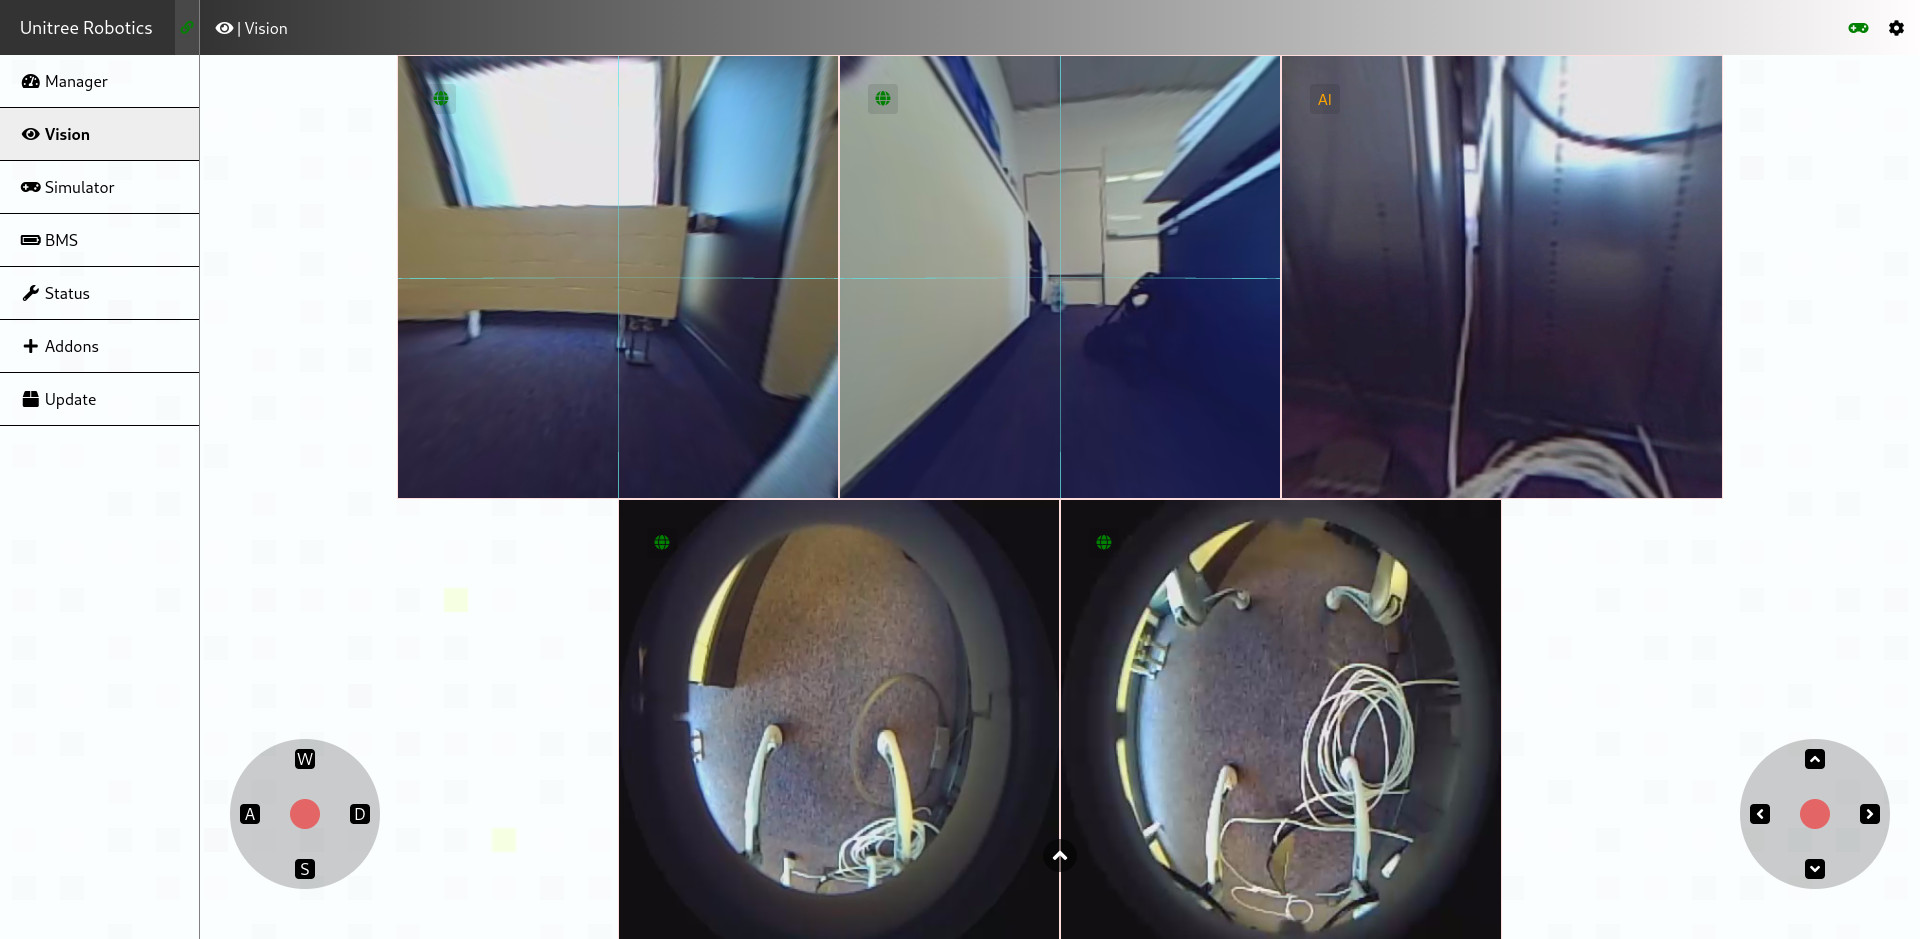
\includegraphics[width=\linewidth]{img/analyse/web-controller}}
    \caption{Bildschirmaufnahme des Web-Controllers}\label{fig:web-controller}
\end{figure}

\myparagraph{Folgefunktion}

Der sogenannte Label-Controller lässt sich genauso wie die Hauptfernbedienung über die Tastenkombination Drücken und
erneutes Drücken und Halten des \texttt{POW}-Knopfes anschalten.
Mit dem Joystick lässt sich der Roboter vereinfacht Steuern.
Die eigentliche Funktion des Label-Controllers ist jedoch die von Unitree Robotics beworbene \emph{Follow Me} Funktion.
Der Controller kommuniziert ständig mit dem Roboter und tauscht Informationen zur angenäherten Position des \gls{go1} relativ
zum Label-Controller aus.
Dies lässt sich in der mobilen App beobachten.
Hierfür muss über die Einstellungen auf den Pfad \texttt{Peripherals > Track Tag} navigiert werden.
Abbildung \ref{fig:follow-me} zeigt die beiden Bildschirmaufnahmen.

\begin{figure}[h]
    \frame{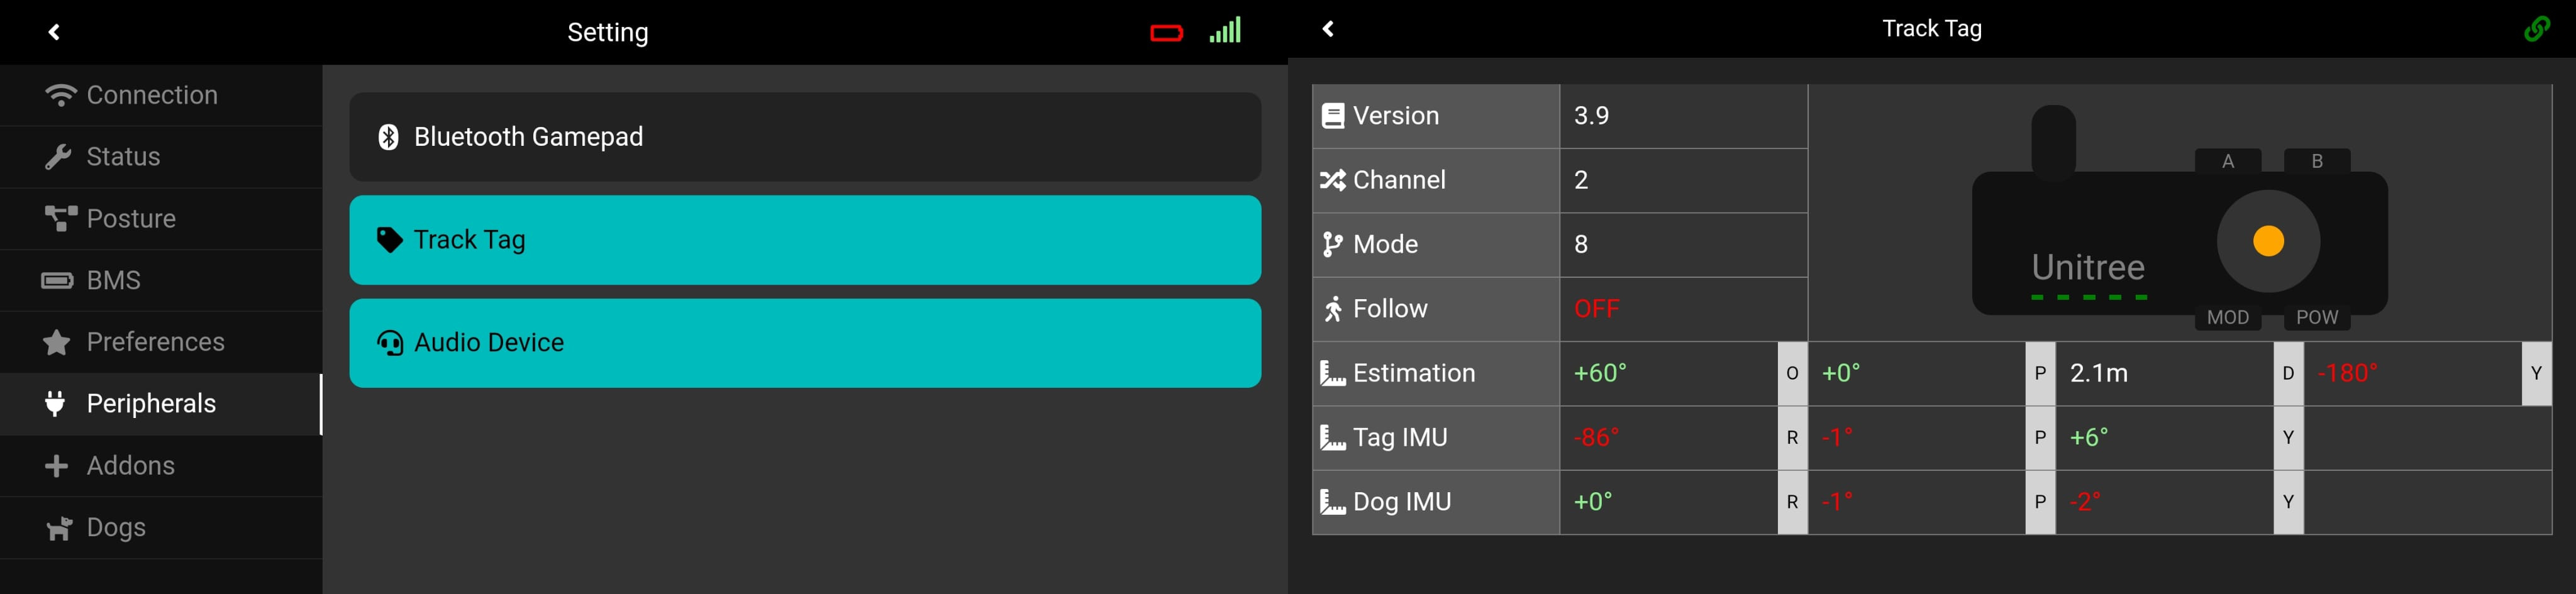
\includegraphics[width=\linewidth]{img/analyse/follow-me}}
    \caption{App-Menüpunkte \texttt{Peripherals > Track Tag} und die Tracking-Übersicht}\label{fig:follow-me}
\end{figure}

Um den Roboter zum Folgen zu bringen, muss der Wert der Option \texttt{Follow} angetippt werden.
Dieser sollte nun von \texttt{OFF} auf \texttt{ON} wechseln.
Danach bewegt sich der Hund immer relativ zum Label-Controller.
Durch die Tasten des Label-Controllers lässt sich das verhalten minimal anpassen.
Tabelle \ref{tab:label-controller-tasten} zeigt fasst die Tastenfunktionen zusammen.

\begin{table}[h]
    \centering
    \begin{tabularx}{\textwidth}{|c|X|}
        \hline
        \textbf{Taste} & \multicolumn{1}{c|}{\textbf{Funktion}} \\ \hline
        POW & \begin{tabular}[c]{@{}l@{}}\num{1} Sekunde Drücken \textrightarrow{} Aufrichten nach Sturz\\ \num{2} mal kurz Drücken \textrightarrow{} Wechsel der Standmodi\\ Stehen \textrightarrow{} Legen \textrightarrow{} Motoren deaktivieren \textrightarrow{} Stehen\end{tabular} \\ \hline
        MOD & \begin{tabular}[c]{@{}l@{}}Kurzes Drücken \textrightarrow{} Folgen deaktivieren\\ \num{2} mal kurz Drücken \textrightarrow{} Wechsel der Modi\\ Langsames Folgen (\num{1,5} m/s) \textrightarrow{} Schnelles Folgen (\num{3} m/s)\end{tabular} \\ \hline
        A & Wechsel Ausweichmodus (nach Test nicht Funktionsfähig) \\ \hline
        B & \begin{tabular}[c]{@{}l@{}}Kurzes Drücken \textrightarrow{} Rotation gegen Uhrzeigersinn um etwa 6\textdegree \\ \num{2} mal kurz Drücken \textrightarrow{} Reset der Rotation auf Standardwert\end{tabular} \\ \hline
    \end{tabularx}\caption{Zusammenfassung der Tastenfunktionen des Label Controllers\label{tab:label-controller-tasten}}
\end{table}

\noindent Anzumerken ist, dass der Label-Controller nicht per Bluetooth mit dem Handy verbunden werden kann.

\subsubsection{Lokales Netzwerk}
\label{subsubsec:lokales-netzwerk}
% Wifi Wlan1 für Netzwerk
% Was wird verbreitet, wer nutzt, App etc

Der Raspberry Pi des \gls{go1} nutzt eines seiner Netzwerk-Schnittstellen, um ein \gls{wlan} zu publizieren.
Ein Blick auf das Autostartmodul \texttt{configNetwork} zeigt, dass hierfür das Interface \texttt{wlan1} verwendet wird.

\lstinputlisting[language=Bash,numbers=left,xleftmargin=\dimexpr2.5em-1pt,framexleftmargin=2em,firstline=35,lastline=38,firstnumber=35]{listing/configNetwork.sh}

\noindent Um weitere Informationen Konfiguration des \gls{wlan} zu finden, muss die \gls{hostapd} Konfiguration in
\texttt{/etc/\allowbreak hostapd/\allowbreak hostapd\allowbreak .conf} betrachtet werden.
Der Service \texttt{\gls{hostapd}} ist ein für Nutzer eines Systems verfügbarer Service für diverse Access Points und
Authentifizierungsserver\footcite{hostapd-doc}.

\lstinputlisting[language=Bash,numbers=left,xleftmargin=\dimexpr2.5em-1pt,framexleftmargin=2em,firstline=18,lastline=22,firstnumber=18]{listing/hostapd.conf}

\noindent Hier ist ersichtlich, dass die \gls{ssid} des \gls{wlan} Access Points der Seriennummer des jeweiligen \gls{go1} entspricht.
Diese ist auf diversen Teilen des Roboters gekennzeichnet.
Das Standardpasswort ist \texttt{00000000} und kann in der Konfigurationsdatei ebenfalls geändert werden.
Nach Neustart des Interfaces \texttt{wlan1} tritt dieses neue Passwort in Kraft.

Ebenfalls hilfreich kann die Funktion einer versteckten \gls{ssid} sein, da der Access Point des \gls{go1} sonst in unmittelbarer
Nähe zum Roboter für jedermann einsichtig wäre, was ein potenzielles Sicherheitsrisiko im regulären Betrieb darstellt.
Hierfür muss lediglich die Zeile \texttt{ignore\_\allowbreak broadcast\_\allowbreak ssid=1} am Ende der Datei hinzugefügt werden.
Die Einstellung bewirkt, dass die Publizierung des \gls{wlan} keine \gls{ssid} bekannt gibt und Verbindungsanfragen ohne eine Angabe der
vollständigen \gls{ssid} ignoriert werden.


\subsubsection{Monitoring}
% App und Webschnittstelle
% todo etwas anderes oder ruas, ist jetz inbetriebnahme
\todo[inline]{Unnötig? Redundant}
\subsubsection{Audio Interfaces}
\label{subsubsec:audio-interfaces}
% Mikrofone und Lautsprecher
% Wie kann ich eigene Dinge abspielen?
% Wo sind /dev/ registriert?
% Was ist installiert? (aplay)
% todo über app wiedergabe

Im Kopf des \gls{go1} ist wie in Abschnitt \ref{par:nano-kopf} beschrieben ein Lautsprecher verbaut.
Ein Blick auf die Hierarchie der verbundenen \gls{usb} Geräte zeigt, dass das Gerät mit der ID \texttt{Dev \num{6}}
die Klasse Audio hat.

\begin{lstlisting}[language=Bash]
unitree@unitree-desktop:~$ lsusb -t | grep Class=Audio
    S|__ Port 4: Dev 6, If 0, Class=Audio, Driver=snd-usb-audio, 12M
    S|__ Port 4: Dev 6, If 1, Class=Audio, Driver=snd-usb-audio, 12M
    S|__ Port 4: Dev 6, If 2, Class=Audio, Driver=snd-usb-audio, 12M
unitree@unitree-desktop:~$ lsusb | grep "Device 006"
Bus 001 Device 006: ID 0d8c:0012 C-Media Electronics, Inc.
\end{lstlisting}

\noindent Der Mount-Point \texttt{/dev/\allowbreak snd/\allowbreak controlC2} des Gerätes lässt sich über den Sym-Link
im Ordner \texttt{/dev/\allowbreak snd/\allowbreak by-id/} auslesen.

\begin{lstlisting}[language=Bash]
unitree@unitree-desktop:~$ ls -l /dev/snd/by-id/
total 0
lrwxrwxrwx 1 root root 12 1x  28 23:58 usb-C-Media_Electronics_Inc._USB_Audio_Device-00 -> ../controlC2
\end{lstlisting}

\noindent Im Folgenden werden zwei Möglichkeiten gezeigt, um den Lautsprecher des Roboters ohne weitere Konfiguration zu nutzen.

\myparagraph{Sprachdurchgabe über App}

Die mobile App für den Roboter ermöglicht es, Mikrofon-Aufnahmen des Gerätes, auf dem die App installiert ist, an den
\gls{go1} zu senden und dann über den Lautsprecher auf der Rückseite des Kopfes abzuspielen.
Hierfür muss die Anwendung zuerst mit dem Roboter verbunden werden.
Danach kann über den Menüpunkt \texttt{Peripherals > Audio Device} auf die Oberfläche zur Konfiguration der Übertragung
zugegriffen werden.
Abbildung \ref{fig:app-audio} zeigt die Übersicht der Audioübertragung.

\begin{figure}[h]
    \frame{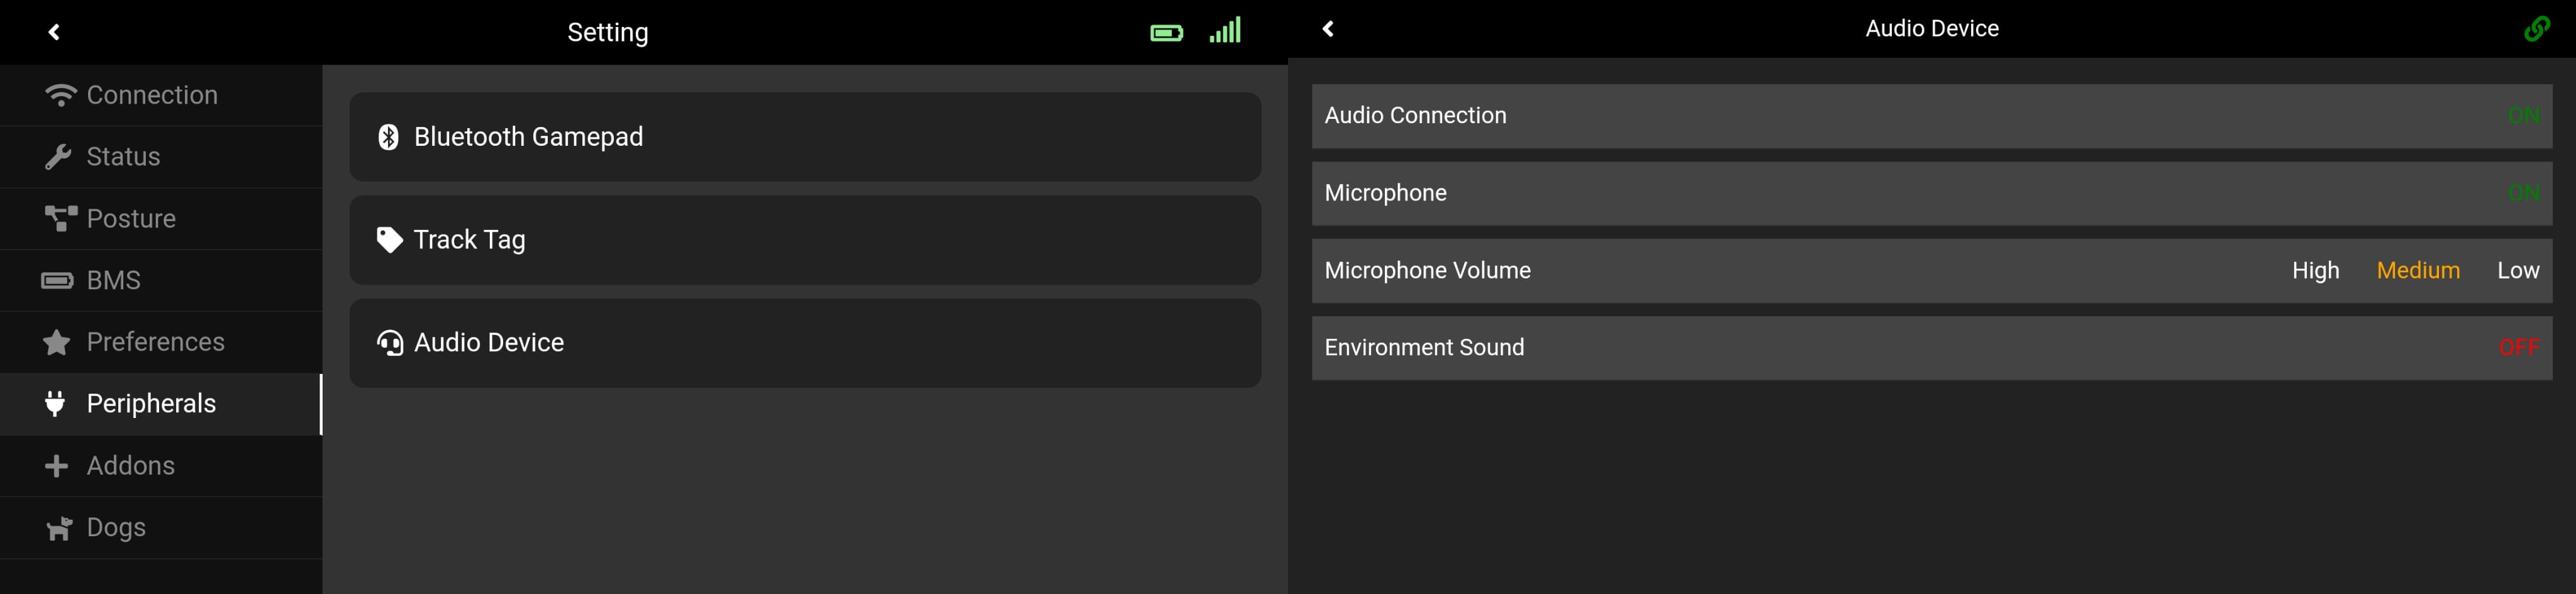
\includegraphics[width=\linewidth]{img/analyse/audio-app}}
    \caption{Überblick über Netzwerkkonfiguration}\label{fig:app-audio}
\end{figure}

Das Icon im rechten oberen Bildrand zeigt an, ob das Audiointerface im Kopf des Hundes erfolgreich verbunden wurde.
Hierfür muss der Autostartprozess \texttt{wsaudio} auf dem Nano noch in Betrieb sein.
Das kann über folgenden Befehl geprüft werden.

\begin{lstlisting}[language=Bash]
unitree@unitree-desktop:~$ ps -aux | grep wsaudio
unitree   8205 95.0  0.4 466312 18360 ?        Rl   00:00   0:23 ./build/wsaudio
\end{lstlisting}

\noindent Sollte dieser Prozess nicht aktiv sein, so kann das Autostartskript manuell ausgeführt werden.

\begin{lstlisting}[language=Bash]
unitree@unitree-desktop:~$ cd /home/unitree/Unitree/autostart/wsaudio/
unitree@unitree-desktop:~/Unitree/autostart/wsaudio$ ./wsaudio.sh &
[1] 9179
[wsaudio] starting ...
unitree@unitree-desktop:~/Unitree/autostart/wsaudio$ ps -ax | grep wsaudio
 9179 pts/0    Rl     3:15 ./build/wsaudio
\end{lstlisting}

\noindent Wichtig ist bei der manuellen Ausführung von Autostartskripten, dass diese aus ihrem Ordner heraus gestartet werden,
da die Skripte selbst oftmals mit relativen Pfaden arbeiten.

In der mobilen Anwendung kann nun der Wert \texttt{Audio Connection} gewählt werden, um diese von \texttt{OFF} auf
\texttt{ON} zu schalten.
Sobald dies auch für den Wert \texttt{Microphone} erledigt wurde, kann über das eingebaute Mikrofon des Handys, auf dem
die Anwendung läuft, Audio aufgenommen werden.
Das Aufgenommene wird dann mit Netzwerk-bedingter Latenz auf dem Lautsprecher abgespielt.

\myparagraph{Abspielen von Audiodateien}

Für das Abspielen von Audiodateien müssen diese erst auf den Nano im Kopf des Roboters kopiert werden.
Hierfür kann die auf den meisten Linux-basierten Betriebssystemen installierte Funktion \texttt{scp} verwendet werden.
Ist der Rechner mit der Datei im Netzwerk des \gls{go1}, so kann folgender Befehl verwendet werden, um die Datei zu kopieren:

\begin{lstlisting}[language=Bash]
sshpass -p 123 scp beispiel.wav unitree@192.168.123.13:~/Music
\end{lstlisting}

Um den Lautsprecher nutzen zu können, müssen alle Prozesse, die diesen blockieren erst beendet werden.
Ab Werk ist das nur der im vorigen Paragraf beschriebene \texttt{wsaudio}-Prozess, der mit dem Kommando \texttt{pkill -f wsaudio}
beendet werden kann.
Danach kann mit dem Befehl \texttt{aplay} die Datei wiedergegeben werden.
Hierfür wird der Gerätename benötigt, welcher mit dem Befehl \texttt{aplay -L}, in dessen Ausgabe nach dem Gerät mit
der Kennung \num{2} gesucht wird.
Die Kennung wurde am Anfang des Kapitels über den Mount-Point erfasst.
Die Ausgabe der Datei \texttt{/proc/\allowbreak asound/\allowbreak cards} zeigt den \gls{usb} Lautsprecher unter dem Index \num{2}.

\begin{lstlisting}[language=Bash]
unitree@unitree-desktop:~$ cat /proc/asound/cards
[...]
 2 [Device         ]: USB-Audio - USB Audio Device
                      C-Media Electronics Inc. USB Audio Device at usb-70090000.xusb-3.4, full speed
\end{lstlisting}

\noindent Die Ausgabe der Datei \texttt{/proc/\allowbreak asound/\allowbreak card2/\allowbreak pcm0p/\allowbreak info} - \texttt{card2} wegen des Indes \num{2} und
\texttt{pcm0p} für das erste \texttt{PLAYBACK} Gerät - zeigt, dass die Karte mit dem Index \num{2} nur einen Kanal hat,
der für das Abspielen verwendet werden kann.

\begin{lstlisting}[language=Bash]
unitree@unitree-desktop:~$ cat /proc/asound/card2/pcm0p/info
card: 2
device: 0
subdevice: 0
stream: PLAYBACK
id: USB Audio
name: USB Audio
subname: subdevice #0
class: 0
subclass: 0
subdevices_count: 1
subdevices_avail: 1
\end{lstlisting}

\noindent Dadurch ergibt sich der direkte Hardwarename des Lautsprechers \texttt{plughw:2,0}
\footnote{\texttt{plug} für gesteckte Hardware \texttt{hw} (z.B. \gls{usb}), \num{2} für den Index, \num{0} für den Kanal (subdevice)},
welcher für folgenden Befehl benötigt wird:

\begin{lstlisting}[language=Bash]
unitree@unitree-desktop:~$ aplay -D plughw:2,0  ~/Music/beispiel.wav
Playing WAVE '/home/unitree/Music/beispiel.wav' : Signed 16 bit Little Endian, Rate 44100 Hz, Stereo
\end{lstlisting}

\noindent Zur einfacheren Handhabung von einem externen Gerät können auch folgende Befehle verwendet werden, insofern das Gerät mit dem Netzwerk
des \gls{go1} verbunden ist:

\begin{lstlisting}[language=Bash]
nlehmann@thinkpadE480 ~ % sshpass -p 123 ssh unitree@192.168.123.13 'pkill -f wsaudio'
nlehmann@thinkpadE480 ~ % sshpass -p 123 ssh unitree@192.168.123.13 'aplay -D plughw:2,0 ~/Music/beispiel.wav'
\end{lstlisting}

\noindent Um die Lautstärke des Lautsprechers anzupassen, stellt die Bibliothek, die auch \texttt{aplay} enthält, ebenfalls die
Funktion \texttt{amixer} zur Verfügung.
Durch den Befehl \texttt{amixer -c 2 set Speaker <0-100>\%}.
Die Option \texttt{-c 2} verweist hier wieder auf die Gerätekennung.\footcite{alsa}

\subsubsection{Kopfbeleuchtung}
\label{subsubsec:led}

Die \gls{led}-Reihen an den beiden Außenseiten des Kopfes sind, wie in Kapitel \ref{sec:roboterarchitektur-und-systemkomponenten}
beschrieben, am Jetson Nano des Kopfes angeschlossen.
Prüft man dort die Funktionen, die über den Autostart gesteuert werden, so fallen zwei Ordner auf -- \texttt{faceLightServer/}
und \texttt{faceLightMqtt/}.
Leider sind die Funktionalitäten beider Skripte als Binärdateien abgelegt und somit nicht ohne weiteres auslesbar.
Auch die Dokumentation des Herstellers weist keinerlei Informationen zu den \gls{led}-Reihen auf.
Der Name des zweiten Ordners weist jedoch auf eine mögliche Funktionalität der Steuerung über MQTT hin.
Um dies zu bestätigen, lässt sich ein MQTT-Explorer verwenden.
Dieser registriert sich als Client beim MQTT-Broker und schreibt alle Nachrichten und veröffentlichten Topics mit.
Mehr zum Thema MQTT gibt es auf der offiziellen Dokumentation des Standards\footnote{https://mqtt.org/}, Beispiele zur Nutzung
des Standards am Roboter in Kapitel \ref{sec:funktionserweiterungen-und-integration}.

Zur Nutzung des MQTT Explorers wird die \gls{ip}-Adresse des Brokers und der Port, auf dem dieser veröffentlicht wird, benötigt.
Für die Adresse kommen nur die \glspl{ip} \texttt{192.168.123.13}, \texttt{...14}, \texttt{...15} und \texttt{...161}
infrage.
Es kann mit der Bibliothek \emph{Nmap} geprüft werden, ob der MQTT-Standardport \texttt{1883} auf einer der registrierten \glspl{ip}
im Netz \texttt{192.168.123.0/24} geöffnet ist.

\begin{lstlisting}
nmap -sS -O -p1883 192.168.123.0/24
\end{lstlisting}

\noindent Die Ausgabe zeigt, dass die beiden \glspl{ip}
\texttt{192\allowbreak .168\allowbreak .123\allowbreak .15} und \texttt{192\allowbreak .168\allowbreak .123\allowbreak .161} den MQTT Port offen haben.
Über den MQTT Explorer wird zunächst der NVIDIA Jetson Xavier NX als Broker getestet.
Die Verbindung funktioniert, jedoch werden weder verfügbare Topics noch Messages ausgegeben.
Ein Test auf dem Raspberry Pi mit der \gls{ip} \texttt{192.168.123.161} zeigt die Ausgabe wie in Abbildung \ref{fig:mqtt-explorer}
dargestellt.

\begin{figure}[h]
    \frame{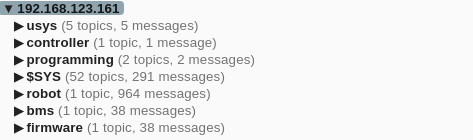
\includegraphics[width=\linewidth]{img/analyse/mqtt-explorer-no-facelight}}
    \caption{Ausgabe eines MQTT Explorers in Verbindung mit dem Raspberry Pi als Broker}\label{fig:mqtt-explorer}
\end{figure}

In den angezeigten Topics sind aktuell noch keine Informationen zu den \glspl{led} zu erkennen.
Dies kann daran liegen, dass das zu dem Topic noch keine Nachrichten versendet wurden, was eine plausible Schlussfolgerung
ist, da die Kopflichter des \gls{go1} standardmäßig ausgeschalten sind.
Ändert man dies nun durch die in der mobilen Anwendung gegebenen Funktion unter dem Menüpunkt \texttt{Preferences}, so
sieht man auch das Topic \texttt{face\_light/color} im MQTT-Explorer, wie in Abbildung \ref{fig:app-mqtt-facelight} dargestellt.

\begin{figure}[h]
    \frame{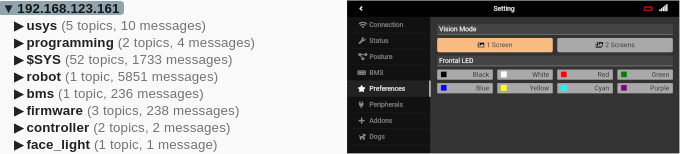
\includegraphics[width=\linewidth]{img/analyse/app-mqtt-facelight}}
    \caption{MQTT Explorer mit Topic \texttt{face\_light/color} (links) und App-Funktion (rechts)}\label{fig:app-mqtt-facelight}
\end{figure}

Die Message Payload kann beispielsweise über das Commandline-Tool \emph{Mosquitto-Client} ausgegeben werden.
Hierfür muss folgender Befehl genutzt werden, um die binäre Payload lesbar auszugeben.
Der genutzte Rechner muss sich hierfür im Netzwerk des \gls{go1} befinden.

\begin{lstlisting}
mosquitto_sub -h 192.168.123.161 -t face_light/color -F %x
ff0000
00ff00
0000ff
\end{lstlisting}

\noindent Die drei Werte in den letzten der Zeilen der Ausgabe sind formatierte Message-Payloads des Topics \texttt{face\_light/color}
und wurden ausgegeben, als in der mobilen Anwendung die drei Farben \emph{Rot}, \emph{Grün} und \emph{Blau} in eben dieser
Reihenfolge eingestellt wurden.
Somit ist herleitbar, dass die \glspl{led} des Roboters über den \emph{RGB}-Farbraum konfigurierbar sind.
Die Mischung aus Rot, Grün und Blau kann hier pro Farbe mit einem Wert von \num{0} - \num{255} eingestellt werden.

Über den Befehl \texttt{mosquitto\_pub} kann nun auch die Farbe des Roboters geändert werden.
Hierfür muss nur das Versenden der Message-Payload in binärer Form beachtet werden.
Folgender Befehl stellt das Kopflicht des \gls{go1} auf Rot um.

\begin{lstlisting}
echo -ne "\xFF\x00\x00" | mosquitto_pub -h 192.168.123.161 -t face_light/color -s
\end{lstlisting}

\noindent Es ist ebenfalls denkbar, die \glspl{led} des Roboters direkt über die \texttt{CP210x UART Bridge} zu steuern, die in Kapitel
\ref{par:nano-kopf} erwähnt wurde.
Dies wurde im Rahmen dieser Arbeit jedoch nicht umgesetzt und kann in Zukunft noch dokumentiert werden.

\subsubsection{Video Streaming}
\label{subsubsec:video-streaming}
% nur möglichkeit, erweiterung in kap 6
% Websockets in Webseite und App
% Welche /dev/ sind vorhanden
% Wer kümmert sich? Pi oder Nanos etc

Der \gls{go1} bietet mit seinen fünf Kameras die Möglichkeit, Bilder seiner Umgebung zu übertragen und es den Nutzern so
zu ermöglichen, den Roboter aus der Entfernung zu steuern.
Die Positionierung, Verteilung und die Mounting-Points der Kameras innerhalb des Roboters, den Recheneinheiten und den
Betriebssystemen wurde bereits in Kapitel \ref{subsec:hardware-architektur} geschildert.
Kurz zusammengefasst sind im Kopf des Roboters zwei Kameras positioniert, nach vorne und nach unten gerichtet.
Beide sind am Jetson Nano innerhalb des Kopfes verbunden.
Die beiden Außenseiten des Rumpfes sind mit zwei Kameras bestückt, die mit dem Jetson Nano m Rumpf des \gls{go1} verbunden sind.
Die letzte Kamera an der Unterseite des Rumpfes ist mit dem Jetson Xavier NX verbunden.
Am Beispiel der nach vorne gerichteten Kamera im Kopf des \gls{go1} soll in diesem Kapitel kurz erläutert werden,
wie auf die Kameras zugegriffen werden kann und wie man von einem verbundenen rechner außerhalb des Roboters auf die Bilder
zugreifen kann.
Die dargestellte Anleitung ist für alle anderen Kameras bis auf etwaige Mounting-Points und \gls{ip} Adressen identisch.

\myparagraph{Zugriff auf Kamerabilder}

Um die Kameras des \gls{go1} nutzen zu können, müssen zuerst alle Prozesse gestoppt werden, die die Geräte selbst blockieren.
Geprüft werden kann dies über den Befehl \texttt{fuser -vm /dev/\allowbreak video1}, hier muss dann nach der Ausgabe nach den Zeilen gesucht werden,
die als \texttt{ACCESS}-Flag den Wert \texttt{m} für \texttt{memory mapped files} haben.
Die Prozesse können dann mit deren Namen beendet werden.

\begin{lstlisting}[language=Bash]
pkill -f point_cloud_nod
pkill -f example_point
\end{lstlisting}

Für den Zugriff auf die Daten der Kamera über den Mount-Point \texttt{/dev/\allowbreak video1} kann das Paket \texttt{ffmpeg}
genutzt werden, das auf allen Ubuntu Systemen des \gls{go1} vorinstalliert ist.
Folgender Befehl inklusive Erläuterung zu den Optionen kann genutzt werden, um per \texttt{ffmpeg} einen Videostream
über \gls{rtsp} auf einen Streaming-Server zu starten.

\begin{lstlisting}[language=Bash]
ffmpeg -nostdin \                  # Keine Interaktion
    -f video4linux2 \              # Input Format
    -i /dev/video1 \               # Input-URL
    -vcodec libx264 \              # Video Kodierung (h264)
    -preset:v ultrafast \          # Kodierungsgeschwindigkeit
    -tune zerolatency \            # Keine H264 B-Frames
    -framerate 5 \                 # Framerate
    -f rtsp \                      # Output Format
    rtsp://<ip:8554|port>/<stream> # Output File/URL
\end{lstlisting}

Weitere Details zur Ausführung und dem Streaming über einen Server werden in Kapitel \ref{sec:funktionserweiterungen-und-integration}
behandelt.

\subsubsection{Sensorik}
% Wo sind Sensoren verbaut?
% Wie kann ich die auslesen?
% Wer ist dafür verantwortlich?

\todo[inline]{Ultraschall testen}

% Sync der Daten minütlich auf Server??
\subsubsection{Batterie Management}
\label{subsubsec:batterie-management}
% Cleveres System
% BMS über MQTT Monitoren
% Was wird angezeigt
% Wie werden Daten interpretiert?
% Wie herausgefunden?

Der Herstellerdokumentation und Werbung ist an einigen Stellen zu entnehmen, dass im \gls{go1} ein intelligentes \gls{bms} verbaut ist.
Dieses ermöglicht es Nutzern, in Echtzeit Informationen zum Stand der Batterie abzugreifen und gegebenenfalls auf die Informationen
zu reagieren.
In der Herstellerdokumentation des Roboters ist nicht dokumentiert, wie die Daten erfasst oder interpretiert werden können,
es wird lediglich auf die beiden Übersichten in der mobilen Anwendung und der Webseite verwiesen, die in Abbildung \ref{fig:bms-app-web}
dargestellt werden.

\begin{figure}[h]
    \frame{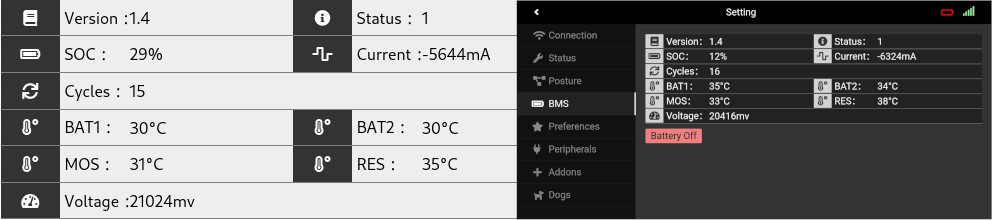
\includegraphics[width=\linewidth]{img/analyse/bms-app-web}}
    \caption{Batterieinformationen in der Webseite (links) und App (rechts)}\label{fig:bms-app-web}
\end{figure}

Die Ausgabe des MQTT-Explorers aus Kapitel \ref{subsubsec:led} beinhaltet ein Topic namens \texttt{bms/\allowbreak state}.
Auch die Prüfung der Webseite über die Entwicklertools innerhalb moderner Browser weisen auf die Bereitstellung der
\gls{bms} Daten über MQTT hin.
Der Dateipfad \texttt{src/\allowbreak plugins/\allowbreak mqtt/\allowbreak receivers/\allowbreak bms\allowbreak Receivers\allowbreak .ts}
und das konfigurierte MQTT-Topic \texttt{bms\allowbreak /state} bestätigen dies.
Gibt man nun die Message-Payloads des Topics aus, so erhält man folgendes Ausgabeformat.

\begin{lstlisting}
mosquitto_sub -h 192.168.123.161 -t bms/state -F %x
0104011bf5e8ffff0f001e1e1f23800da00d20002000a00da00da00d20002000800d
\end{lstlisting}

Man kann über die Entwicklertools der modernen Browser die Struktur der Daten zurückverfolgen.
Zeile \num{14} zeigt die Umwandlung der Message-Payload aus einem \texttt{Byte\allowbreak Buffer} in ein \texttt{Uint8Array}.
Laut der JavaScript-Dokumentation ist ein \texttt{Uint8Array} ein Array aus \num{8}-bit unsigned Integer\footcite{uint8array}.
Somit können je zwei Ziffern der hexadezimalen Ausgabe des \gls{bms} als ein Wert des Arrays interpretiert werden.
Die Zeilen \num{14} bis \num{17} und Zeile \num{20} in Listing \ref{lst:bms-reverse} zeigen die Umwandlungen der \num{8}-bit Integer.

\begin{lstlisting}[language=JavaScript,numbers=left,xleftmargin=2.5em,framexleftmargin=2em,firstnumber=14,label={lst:bms-reverse}]
const uint8s = new Uint8Array(message);
data.bms.version = uint8s[0] + "." + uint8s[1];
data.bms.status = uint8s[2];
data.bms.soc = uint8s[3];
data.bms.current = dataView.getInt32(4, true);
data.bms.cycle = dataView.getUint16(8, true);
data.bms.temps = [uint8s[10],uint8s[11],uint8s[12],uint8s[13]];
for (let i = 0; i < 10; i++) {
  data.bms.cellVoltages[i] = dataView.getUint16(14+i*2, true);
}
data.bms.voltage = data.bms.cellVoltages.reduce((a,c) => a+c);
\end{lstlisting}

\noindent Die Dokumentation der Klasse \texttt{DataView} zeigt, das die Funktionen \texttt{getInt32()} und \texttt{getUint16()}
folgenden Syntax haben\footcite{dataview}.

\begin{lstlisting}[language=JavaScript]
getInt32(byteOffset, littleEndian)
getUint16(byteOffset, littleEndian)
\end{lstlisting}

Somit wird in Zeile \num{18} ein \num{4}-Byte Integer ab dem fünften Byte der Message-Payload ausgelesen, in den Zeile
\num{19} ein \num{2}-Byte Integer ab dem neunten Byte und zehn weitere ab dem fünfzehnten Byte der Payload gelesen.
Die zehn letzten \num{2}-Byte Integer werden zu einer Gesamtzahl addiert.
Durch die Auswertungen der Webseite ergibt sich folgender Überblick über das Format der Payload.
Das verwendete Beispiel ist die oben gezeigte Ausgabe des Befehls \texttt{mosquitto\_\allowbreak sub}.

\begin{table}[h]
    \centering
    \begin{tabularx}{\textwidth}{|X|X|X|X|XX|}
        \hline
        \textbf{Byte} & \textbf{Format} & \textbf{Inhalt} & \textbf{Beispiel} & \multicolumn{2}{c|}{\textbf{Konvertierung}} \\ \hline
        0-1 & 2 x uint8 & Version & 01, 04 & \multicolumn{2}{c|}{v1.4} \\ \hline
        2 & uint8 & Status & 01 & \multicolumn{2}{c|}{1} \\ \hline
        3 & uint8 & State of Charge & 1b & \multicolumn{2}{c|}{27 \%} \\ \hline
        4-7 & int32 & Strom & f5e8ffff & \multicolumn{2}{c|}{-5899 mA} \\ \hline
        8-9 & uint16 & Zyklus & 0f00 & \multicolumn{2}{c|}{15} \\ \hline
        10-13 & 4 x uint8 & Temperaturen & \begin{tabular}[c]{@{}c@{}}1e, 1e,\\ 1f, 23\end{tabular} & \multicolumn{2}{c|}{\begin{tabular}[c]{@{}c@{}}30 \textdegree C, 30 \textdegree C\\ 31 \textdegree C, 35 \textdegree C\end{tabular}} \\ \hline
        14-33 & 10 x uint16 & Zell-Spannung & \begin{tabular}[c]{@{}c@{}}800d, a00d,\\ 2000, 2000,\\ a00d, a00d,\\ a00d, 2000,\\ 2000, 800d\end{tabular} & \multicolumn{1}{c|}{\begin{tabular}[c]{@{}c@{}}3456 mV, 3488 mV,\\ 32 mV, 32 mV,\\ 3488 mV, 3488 mV,\\ 3488 mV, 32 mV,\\ 32 mV, 3456 mV\end{tabular}} & \begin{tabular}[c]{@{}c@{}}\textbf{Summe:}\\ 20,992 V\end{tabular} \\ \hline
    \end{tabularx}
    \label{tab:bms-format-matrix}
\end{table}

Im Kapitel \ref{sec:funktionserweiterungen-und-integration} wird gezeigt, wie die Informationen des \gls{bms} sinnvoll
ausgelesen und verwertet werden können.

